\setauthor{Benjamin Ecker}

Hier werden alle Funktionalitäten des Frontends erklärt und wie es mithilfe der verschiedenen Libraries arbeitet.  Anfangs wird die Ordnerstruktur erklärt um sich erstmal in einer Angular App zurechtzufinden.

\section{Ordnerstruktur}
\begin{figure}[H]
    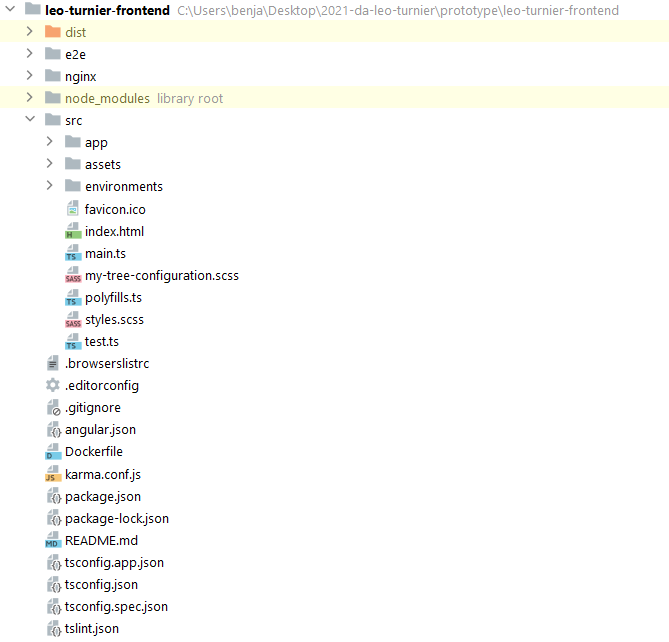
\includegraphics[scale=0.8]{pics/frontend/angular_file_structure.PNG}
    \caption{Angular Ordnerstruktur}
\end{figure}

Bei der Erstellung einer Angular Applikation wird schon fast die gesamte Ordnerstruktur festgelegt. Bis auf ein paar Ausnahmen wie der Nginx Ordner, oder die zwei in Gelb markierten Ordner,
welche nach dem dem Laden bzw. Builden generiert werden, hat sich hier nichts getan.
Wie an den meisten Filenamen schon zu erkennen ist befinden sich auf dieser Ebene so fast nur Files, die zur Konfiguration nötig sind. Das wichtigste File dabei ist "package.json".

\begin{figure}[H]
    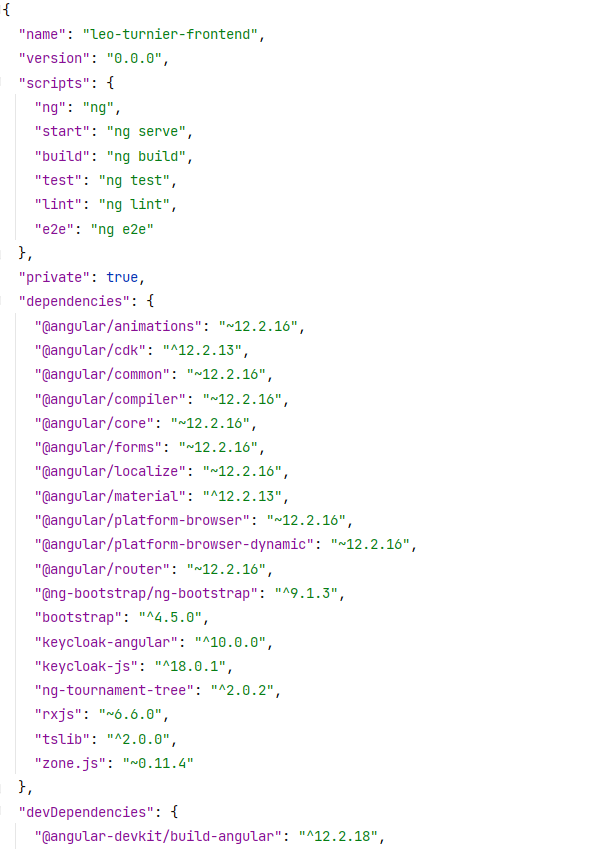
\includegraphics[scale=0.6]{pics/frontend/package_json.PNG}
    \caption{package.json}
\end{figure}

Hier werden alle Metadaten, Scripts und Dependencies der App aufgelistet.
Bei den Dependencies unterscheidet man zwischen Dependencies und DevDependencies.
\begin{itemize}
    \item Dependencies werden transitiv installiert: Wenn A B benötigt und B C benötigt, wird C installiert, sonst könnte B nicht funktionieren und A auch nicht.
    \item DevDependencies werden nicht transitiv installiert. Wir brauchen z.B. B nicht zu testen, um A zu testen, also können die Testabhängigkeiten von B weggelassen werden.
\end{itemize}

Um diese Dependencies auch nützen zu können muss bei jedem Angular Projekt "npm install" ausgeführt werden um diese zu laden.
Danach werden sie dann im Ordner node\_modules gespeichert.
Dieser sollte, aber vor jeder Weitergabe gelöscht werden,oder wie zum Beispiel in Git im ".gitignore" inkludiert werden, da dieser mit Abstand am speicherintensivsten ist. 

\newpage
Auch wenn Angular eine große Anzahl an Ordnern und Files bietet geschieht wahrscheinlich 99\% der Arbeit eines Angular-Projekt im app Ordner.
Dieser enthält alle Components sowie Klassen die für die Applikation benötigt werden.

\begin{figure}[H]
    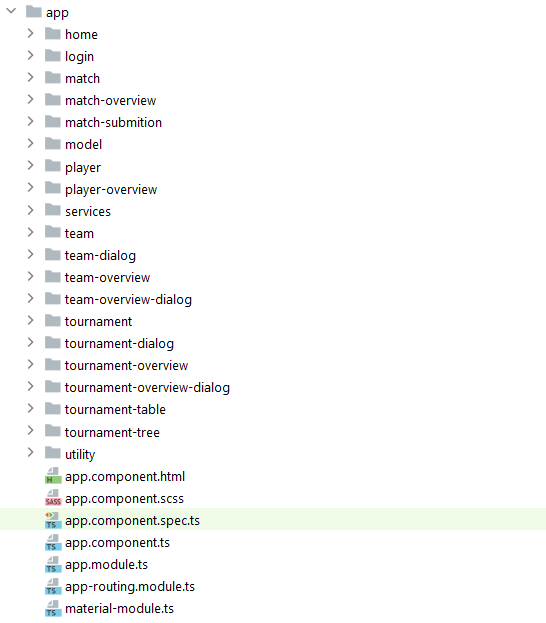
\includegraphics[scale=0.6]{pics/frontend/app_folder.PNG}
    \caption{App Ordner}
\end{figure}

Um ein bisschen Ordnung ins Chaos zu bringen kann man diese Files bzw Ordner in drei Kategorien unterteilen:
\begin{itemize}
    \item App Components: Alle Files die mit app anfangen
    \item Hilfklassen: model, services, utility, material-module.ts
    \item Components: Alle restlichen Ordner.
\end{itemize}

\subsection{App Components}
\subsubsection{Modules und Routing}

Modules und Routing sind der Kern einer Angular App. Hier laufen alle Components zusammen und 
Libraries werden über Imports eingebunden. Im Routing findet unter routes ein Array mit allen paths, sowie deren Components. Mit @NgModule wird das App-Modul erstellt.
Dort findet man dann auch alle Abhängigkeiten und Komponenten, die dieses Modul enthält. Um einen guten Überblick über alle Modules zu haben, wurden für die große Anzahl an AngularMaterial Modules ein eigens Module erstellt.
Beim Laden dieses Moduls wird der AppComponent gestartet. 
\cite{implementation-angular-1}

\begin{figure}[H]
    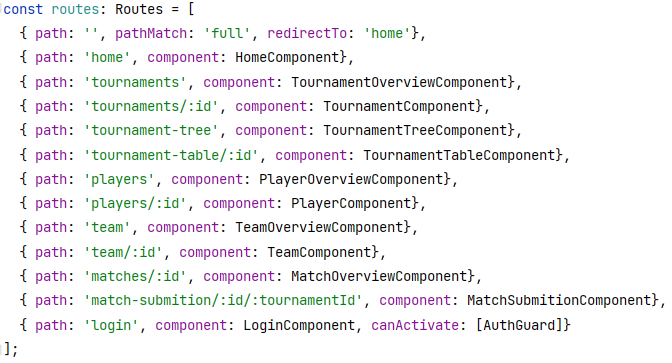
\includegraphics[scale=0.5]{pics/frontend/routes.PNG}
    \caption{routes in app-routing.module.ts}
\end{figure}

\begin{figure}[H]
    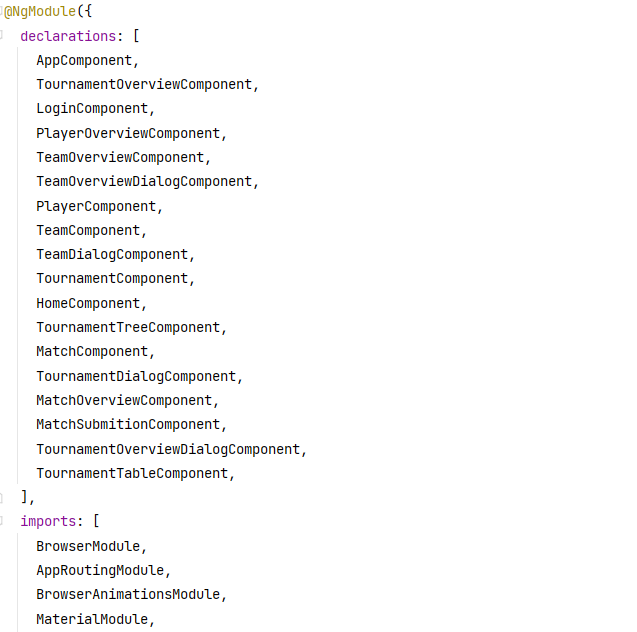
\includegraphics[scale=0.5]{pics/frontend/app_module.PNG}
    \caption{@NgModule in app.module.ts}
\end{figure}

\subsubsection{App-Component}

Die App Component ist der "Vater" jeder Angular App. Sie enthält alle anderen Child-Components und ist jederzeit sichtbar.
Daher eigent Sie sich perfekt für eine Tool- und Navbar. 
Wie alle Component besteht Sie aus 4 Files:
\begin{itemize}
    \item TypeScript (.ts): Ist der Code-Behind und enthält die gesamte Business Logik der Component. 
    \item HTML
    \item SCSS: Durch SCSS wird die Schreibweise von CSS vereinfacht und Variablen fest definiert.
    \item spec.ts: Die spec-Dateien sind Unit-Tests für den Sourcecode. Die Konvention für Angular-Anwendungen ist es, eine .spec.ts-Datei für jede .ts-Datei zu haben. \cite{implementation-angular-2}
\end{itemize}

\subsection{Hilfsklassen}
\subsubsection{Model}
Hier sind alle Klassen der App untergebracht. Bis auf ein paar Abweichung findet man hier das gleiche Datenmodel wie im Backend(7.1) wieder.
Da Angular mit Typescript verwendet wird, können für diese Klasse type checking verwendet werden (in vielen Fällen können stattdessen auch ein Interface verwendet werden)

\begin{figure}[H]
    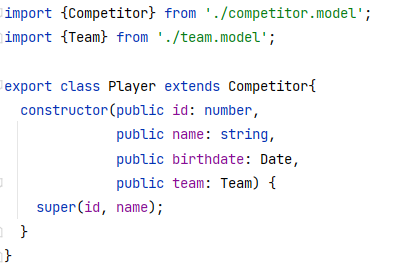
\includegraphics[scale=0.7]{pics/frontend/player_model.png}
    \caption{player.model.ts}
\end{figure}

\subsubsection{Services}
Components sollten Daten nicht direkt abrufen oder speichern. Sie sollten sich auf die Darstellung von Daten konzentrieren und den Datenzugriff an einen Service delegieren. In dem Ordner services befindet sich daher der gesamte Service, aufgeteilt in Aufgabenbereiche.
Jeder Service ist dabei gleich aufgebaut. Damit Angular den Service in eine Component injecten kann muss vorher ein Provider eingetragen werden. Ein Provider ist etwas, das einen Service erstellen oder bereitstellen kann.
Um sicherzustellen, dass der Service diesen anbieten kann, registrieren Sie ihn beim Injektor. Der Injektor ist das Objekt, das den Provider auswählt und dort injiziert, wo die Anwendung ihn benötigt.
Standardmäßig trägt Angular hierführ 'root' ein. Wenn ein Dienst auf Root-Ebene bereitgestellt wird, erstellt Angular eine einzelne, gemeinsam genutzte Instanz des Services und injiziert diese in jede Klasse, die danach fragt. \cite{implementation-angular-3}

Um Daten auf die Daten des Backends zugreifen zu können wird die Client-HTTP-API verwendet, welcher zugleich noch Features für Error-Handling und Typed Response Objects  bereitstellt. \cite{implementation-angular-4}

Da nicht jeder Nutzer von LeoTurnier Zugriff zu allen Daten haben darf, wird dazu noch ein Keycloak-Service verwendet der für jeden Request einen Authentication-Token zur Verfügung stellt.
Damit dieser Service funktioniert muss man zuerst den Keycloa-Server mit dem Frontend verbinden.

\begin{figure}[H]
    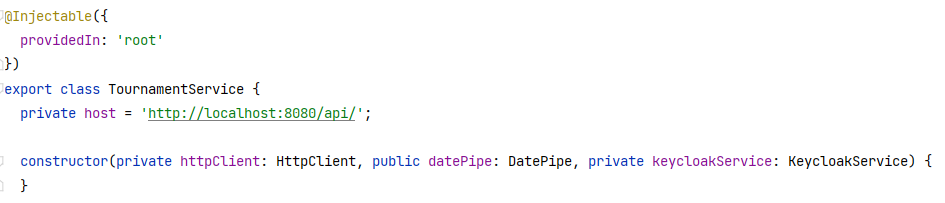
\includegraphics[scale=0.6]{pics/frontend/service.PNG}
    \caption{tournament.service.ts}
\end{figure}

\begin{figure}[H]
    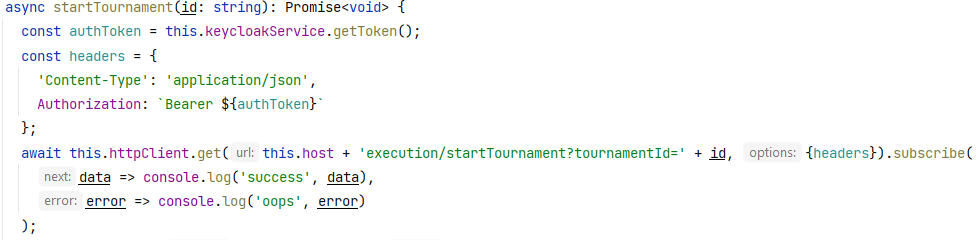
\includegraphics[scale=0.6]{pics/frontend/example_request.PNG}
    \caption{Beispiel Request: startTournament}
\end{figure}

\subsubsection{Utility - Keycloak}

In diesem Ordner befinden sich alle nötigen Files für  eine funktionierde Verbindung mit Keycloak.
Für die Initialisierung des KeycloakService ist eine Methode im "app.init.ts" zuständig. Als Vorlage diente hierführ
das Tutorial des Keycloak-Angular Module von Maurico Vigolo
\cite{sysarch-keycloak-angular-1}

\begin{figure}[H]
    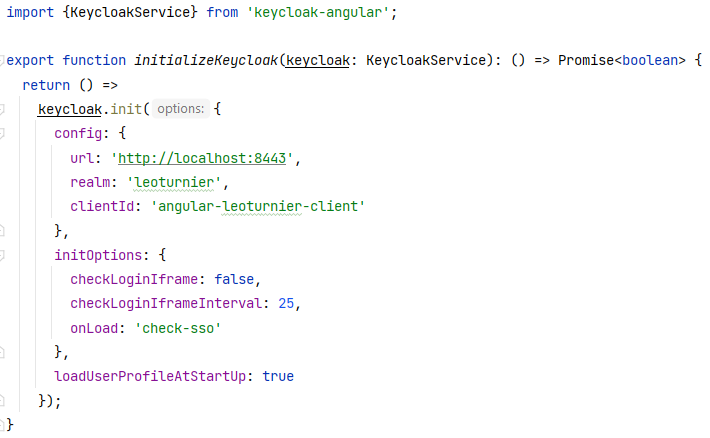
\includegraphics[scale=0.6]{pics/frontend/app_init.PNG}
    \caption{app.init.ts}
\end{figure}

Wie im Screenshot zusehen befindet sich hier eine Konfiguration für einen Client von Keycloak. Dieser kann dann an Keycloak eine Anforderung stellen, um einen Benutzer zu authentifizieren, Identitätsinformationen einzuholen, oder einen Zugriffstoken anzuforden.
Der Client muss direkt im Keycloak mit der Administration Console erstellt werden und muss mit der Konfiguration und der Frontend URL genau übereinstimmen.

\begin{figure}[H]
    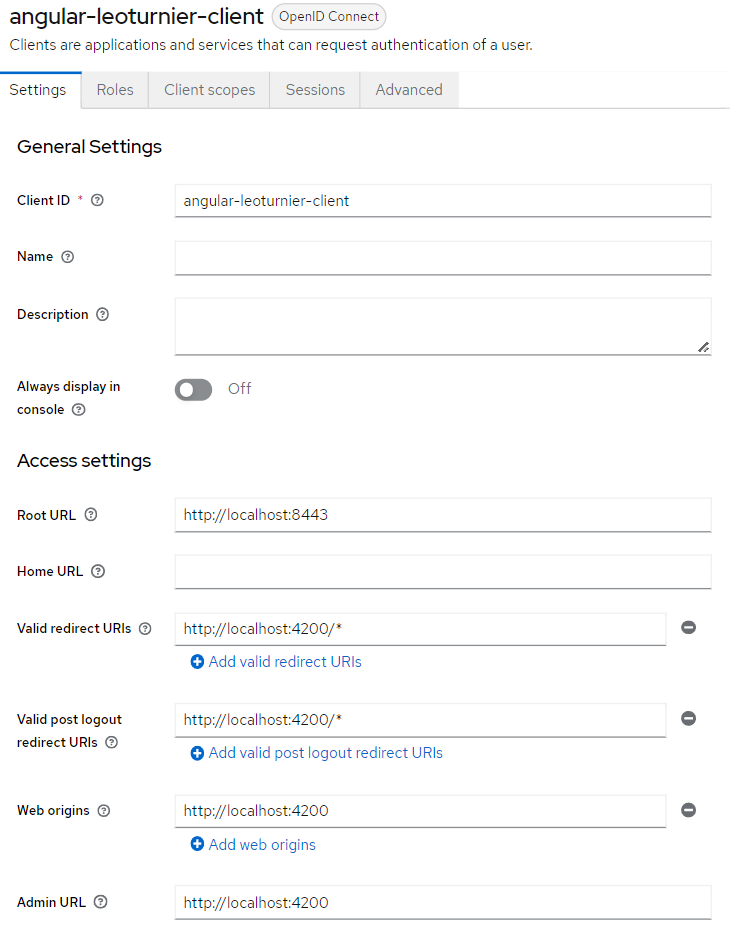
\includegraphics[scale=0.7]{pics/frontend/keycloak_client.PNG}
    \caption{Keycloak-Frontend Client}
\end{figure}

\subsection{Components}
Components sind die UI-Bausteine einer jeden Angular App. Wie vorher schon erwähnt sind alle anderen Komponenten Child-Components der App-Component und bilden somit Component-Tree.
LeoTurnier ist hierbei sehr simpel gehalten und besitzt einen fast komplett flachen Baum. 
Auch wenn jede Component einzigartig ist und ihren eigenen Funktionalitäten hat funktionieren haben sie viele Gemeinsamkeiten:

\subsubsection{Service}
Um beispielsweise eine Tabelle ein Formular zu füllen braucht jede Component mindestens einen Service. Dieser wird im Konstruktor injiziert, aber kann in ihm noch nicht verwendet werden. In den meisten Fällen wie bei einer Tabelle müssen die 
Daten aber schon zu Begin bereitgestellt werden. Hier kommt die Methode ngOnInit ins Spiel.

\subsubsection{OnInit}
Um ngOnInit verwenden zu könenn muss vorher das die Component vorher OnInit implementieren. Im Grunde handelt es sich hierbei nur um eine Lifecycle-Hook, welche Angular selbst verwaltet.
Die Methode wird dann nur zur Initialisierung der Component aufgerufen, wie uns der Name schon verrät. Somit wird sofort nach dem Konstruktor die Methode aufgerufen. Dabei können Daten können schon vor dem Start der Component beschaffen werden und danach vielleicht Tabelle befüllt werden. \cite{implementation-angular-5}

\begin{figure}[H]
    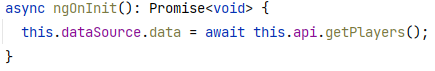
\includegraphics[scale=0.8]{pics/frontend/example_ngOnInit.PNG}
    \caption{Beispiel Router-Call aus player-overview.component.ts}
\end{figure}
\subsubsection{Router}
Will man jetzt in dieser Tabelle die beispielsweise mit Spielern einen bearbeiten, ist eine eigene Component nötig. Um es also für eine Component zu ermöglichen auf eine andere Component zu navigieren, ist ein sogenannter Router nötig. Dieser wird genau wie der Service injiziert und gehört zum RouterModule. 
Nun kann der Router mithilfe der Routes im "app-routing.module.ts" den Benutzer zu einer anderen Component navigieren und für diese auch Parameter mitgeben.

\begin{figure}[H]
    
\includegraphics[scale=1]{pics/frontend/example_navigation.PNG}
    \caption{Beispiel Router-Call aus player-overview.component.ts}
\end{figure}

Diese Parameter müssen dann auch von der anderen Component gespeichert werden. Hier schafft der ActivatedRouter abhilfe. Das Prozedere ist hierbei genau gleich wie beim Router und der Auruf kann sofort im Konstruktor stattfinden.

\begin{figure}[H]
    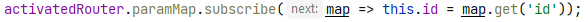
\includegraphics[scale=1]{pics/frontend/example_activatedRouter.PNG}
    \caption{Beispiel ActivatedRouter-Call aus player.component.ts}
\end{figure}

\section{Tournament-Tree}

Eine ansprechensden Aufgaben des Frontend ist die Visualisierung der Turniere, vor allem die des Elimination stellen eine große Herausforderung dar. Darum verwendet das Frontend für Erstellung eines optisch ansprechenden Turnierbaums das Module NgTournament was diese Aufgabe massiv erleichtern soll. \cite{implementation-angular-6}

Die hierführ benötigten Components finden sich im Order Match, Tournament-Tree und Home.

\subsubsection{Home}
Zuallererst braucht NgTournament Information über den gesamten Turnierverlauf. Diese müssen in Form eines NggtTournament vorhanden sein, welches wiederum aus Rounds und Matches besteht. Den Algorithmus hierführ stellt NgTournament bereit, dieser muss nur auf das eigene Datenmodel geändert werden und schon sollte es gehen,
da NgTournament aber leider nur fertig gespielte Turniere visualisieren kann, musste der Algorithmus noch so ergänzt werden, dass bei noch nicht gespielten Matches als "Austehend" aufgeführt werden. 

\begin{figure}[H]
    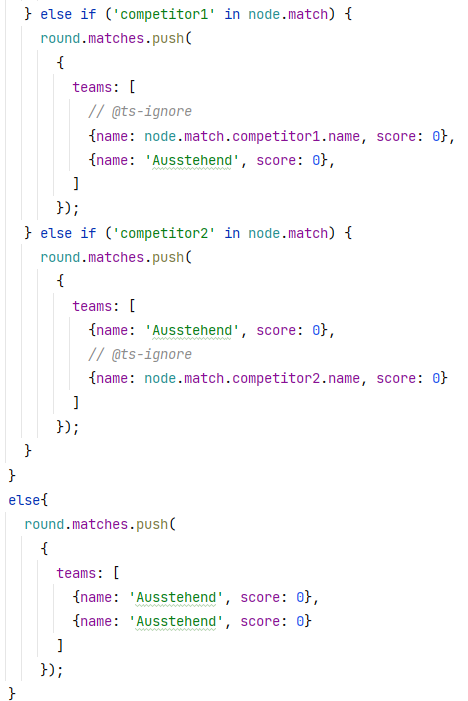
\includegraphics[scale=0.7]{pics/frontend/ausstehende_matches.PNG}
    \caption{hinzufügen ausstehender Matches in showTree(Home-Component)}
\end{figure}

\subsubsection{Tournament-Tree \& Home}
Nachdem das Tournament als NggtTournament vorhanden ist wird dieses an das Tournament-Tree Component geleitet, sie komplett von NgTournament bereitgestellt und muss auch nicht mehr bearbeitet werden. 
Nun rendert die Tournament-Tree Component mithilfe der Match Component als Template, welche auch vollständig bereitgestellt wird, den kompletten Turnierbaum.

\bigskip
\begin{figure}[H]
    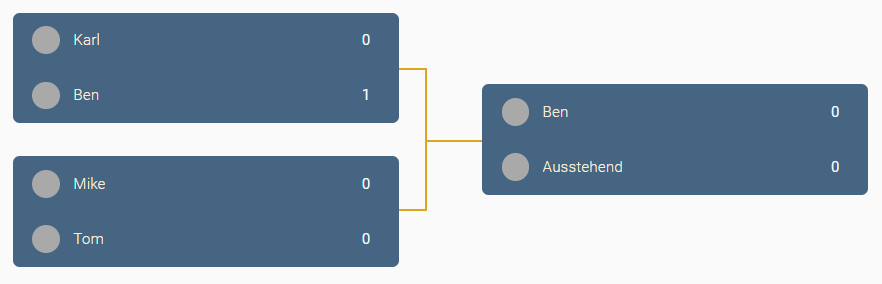
\includegraphics[scale=0.7]{pics/frontend/tournament-tree.PNG}
    \caption{Turnierbaum}
\end{figure}

\subsubsection{Styling}
Das Styling für den Turnierbaum wird bereits beim Laden des NgTournament hinzugefügen. Doch mit da der Baum auf weißen Hintergrund platziert ist passte es besser, wenn der Turnierbaum auch einen weißen Hintergrund besitzt.
Um das grundlegende Styling zu überschreiben schafft das File "my-tree-configurations.scss" abhilfe, welches nur im "style.scss" vor "ng-tournament-tree/styles/ngtt-styles" imported werden muss.

\begin{figure}[H]
    
\includegraphics[scale=1]{pics/frontend/my_tree_css.PNG}
    \caption{my-tree-configurations.scss}
\end{figure}

\begin{figure}[H]
    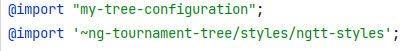
\includegraphics[scale=1]{pics/frontend/style_css.PNG}
    \caption{style.scss}
\end{figure}